% vim: set filetype=tex:ai:et:sw=4:ts=4:sts=4:tw=80
%----------------------------------------------------------------------------------------
%	PACKAGES AND OTHER DOCUMENT CONFIGURATIONS
%----------------------------------------------------------------------------------------

\documentclass{article}

\usepackage[utf8]{inputenc}
\usepackage{fancyhdr} % Required for custom headers
\usepackage{extramarks} % Required for headers and footers
\usepackage{graphicx} % Required to insert images
\graphicspath{ {./pic/} }
\usepackage[backend=bibtex,style=numeric,sorting=none]{biblatex}
\usepackage{url}
\usepackage{mathtools}
\usepackage{hyperref}

% Margins
\topmargin=-0.45in
\evensidemargin=0in
\oddsidemargin=0in
\textwidth=6.5in
\textheight=9.0in
\headsep=0.25in

\linespread{1.1} % Line spacing

%----------------------------------------------------------------------------------------
%	TITLE
%----------------------------------------------------------------------------------------

\title{
\textmd{IA158 Real Time Systems}\\
\textmd{\textbf{Legway}}
}

\author{\textbf{Jan Dupal, Adrian Farmadin, Peter Kotvan, Vít Šesták}}
\date{11. 5. 2014} % Insert date here if you want it to appear below your name

\bibliography{./bib/bibliography.bib}

%----------------------------------------------------------------------------------------

\begin{document}

\maketitle

\section{Introduction}

Our project is inspired by Segway, two-wheeled, self-balancing, battery-powered
vehicle. \cite{segway} \cite{wseg} As the Lego robotic set did not contain
gyroscopes we used light sensor for measuring the tilt of the robot as can be
seen on figure~\ref{fig:legway}. The sensor is located under the Lego brick.

\begin{figure}[h]
    \centering
    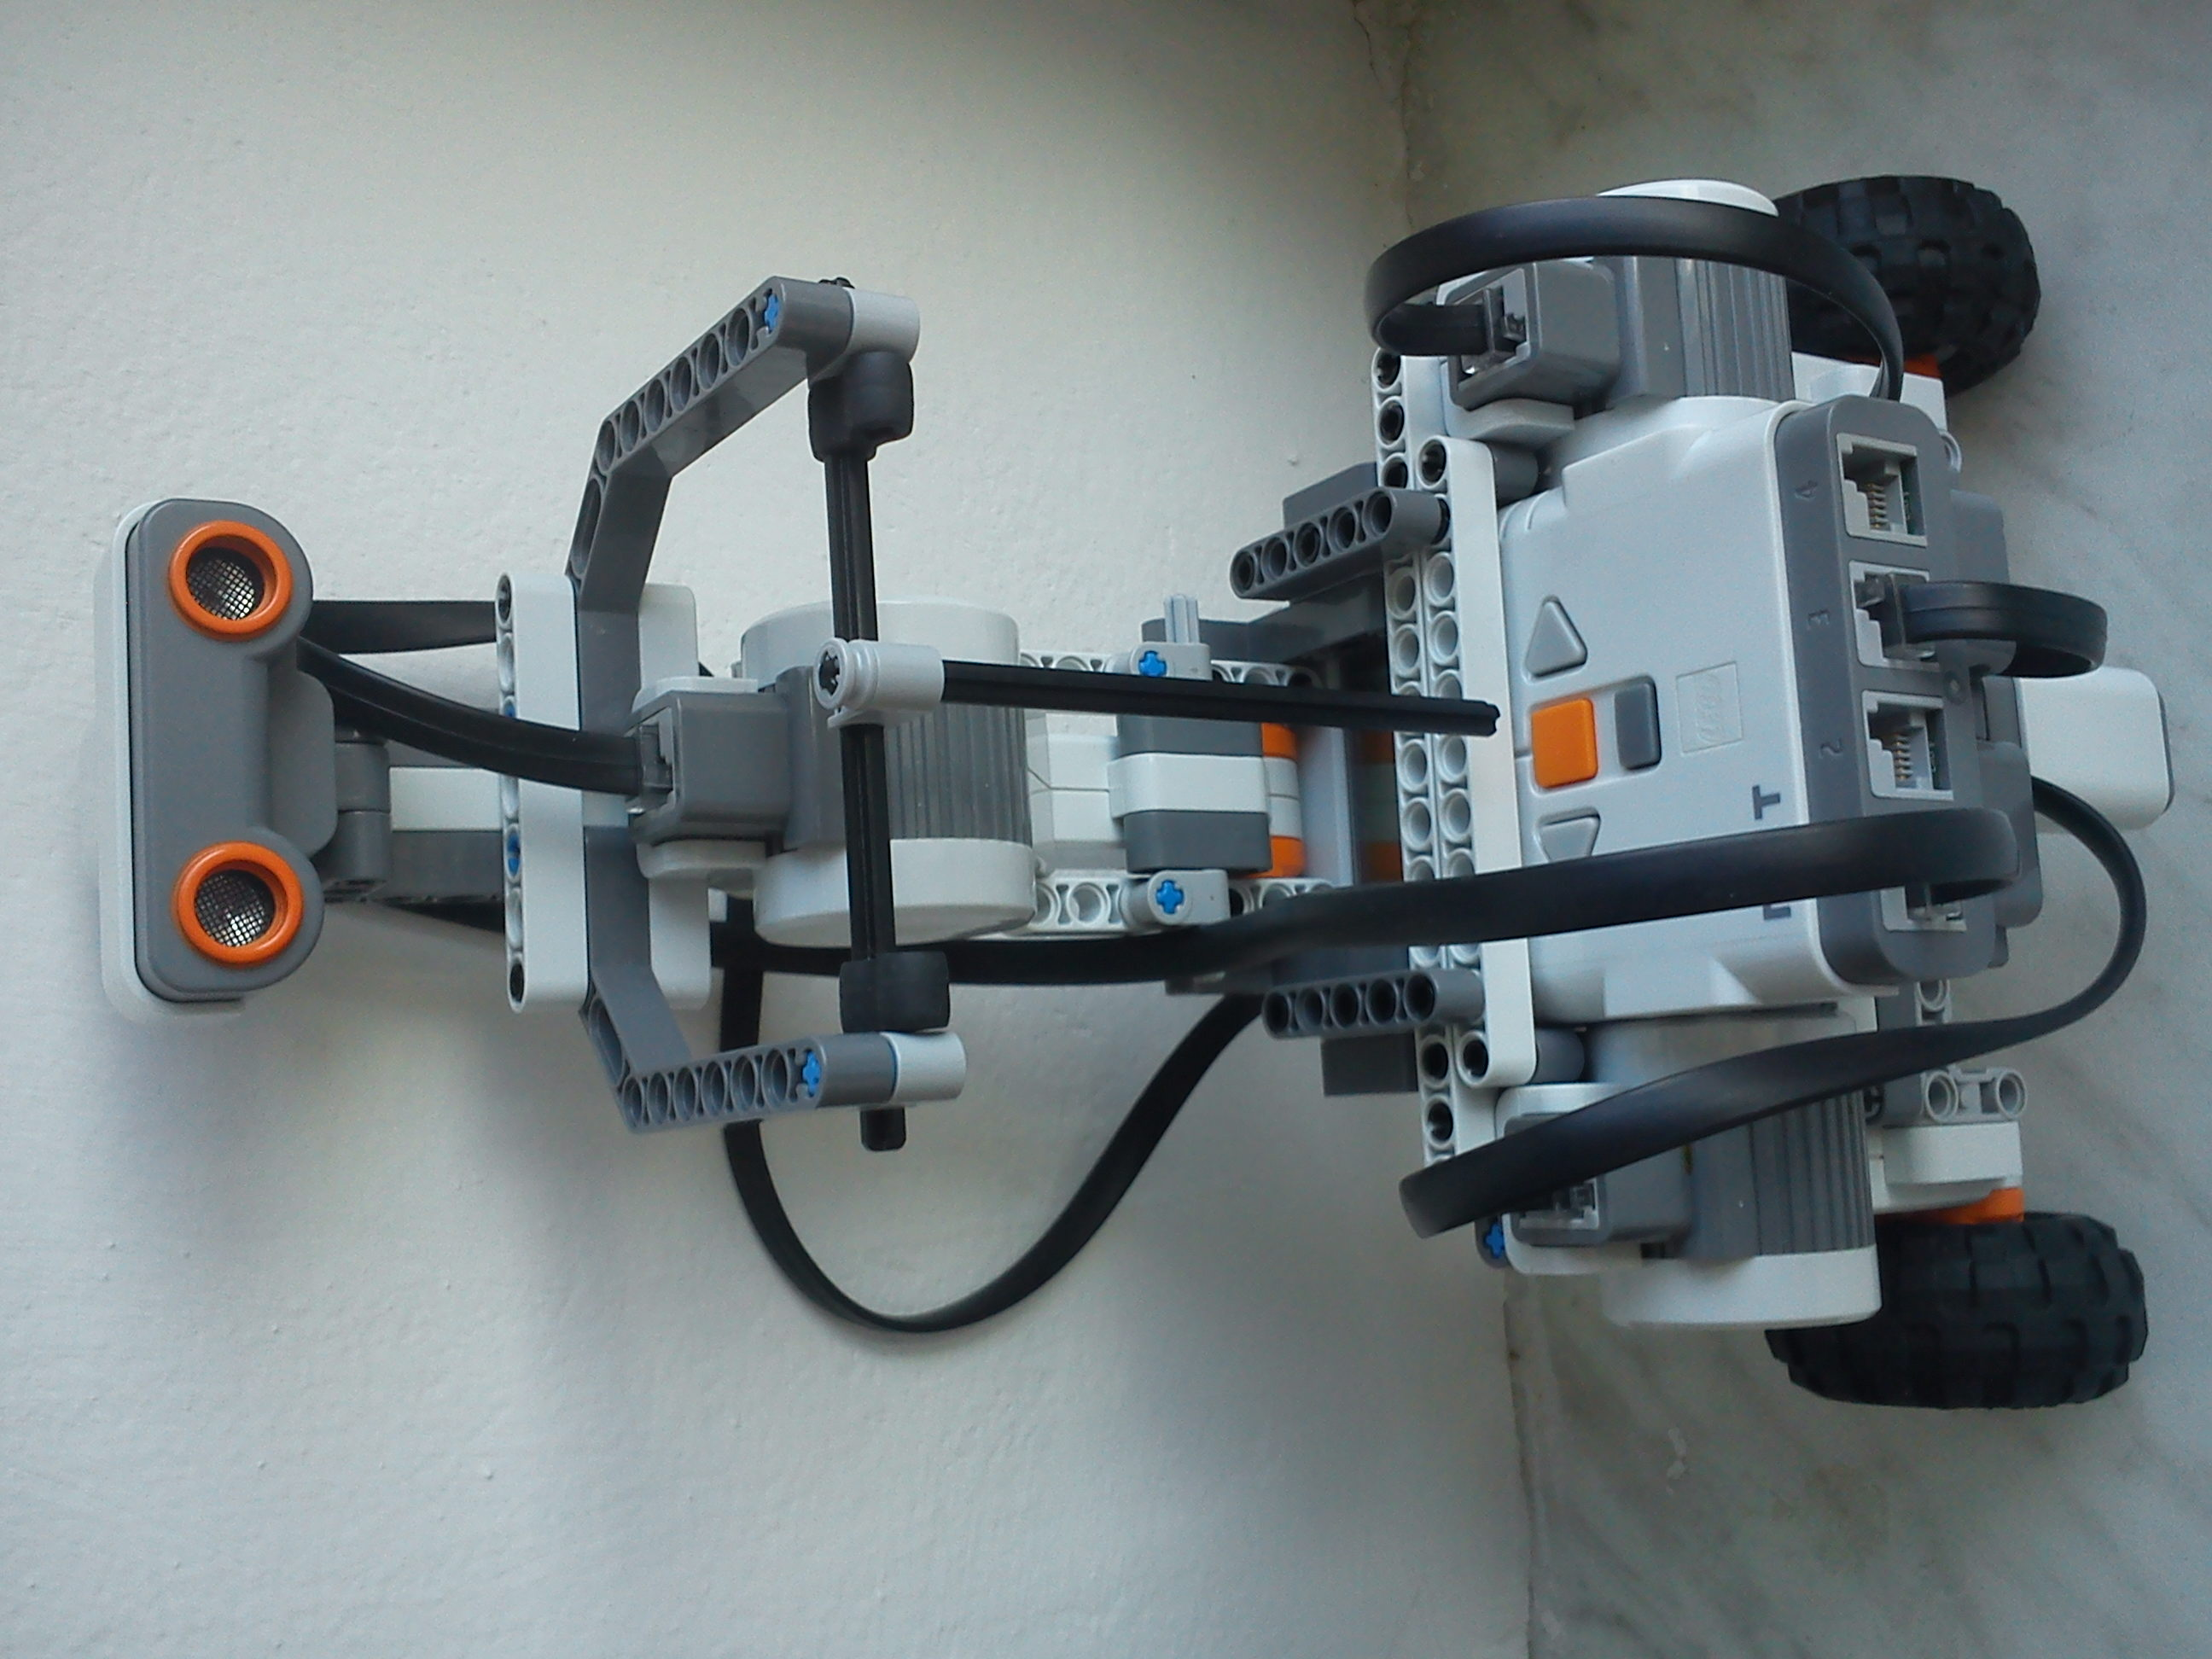
\includegraphics[width=7cm, angle=270]{legway}
    \caption{Legway}
    \label{fig:legway}
\end{figure}

The communication with Lego brick is done over bluetooth. Initially we intended
to use ultrasonic sensor to avoid obstacles but later we decided to remove
unnecessary parts to lower the centre of gravity to solve our problems with
balancing.

For different parts of the project our team used different programming
languages. The main program of the robot is written in NXC \cite{nxc} which is a
language very similar to C. Testing module for bluetooth communication is
written in Ruby and finally the application for controlling the segway is
written in Scala.

Unfortunately during our work on this project we experienced display failure on
Lego brick two times. This caused delay in our work and the second malfunction
prevented us from merging the codebases of team members and from enough
experimentation with controller parameters as our team used the display for
debugging purposes.

\section{Controller}

Control theory is a branch of science that studies the behavior of dynamical
systems and describes the ways of controlling them. To enable our robot to
balance itself we had to implement basic PID controller with with feedback loop.
Figure~\ref{fig:loop} shows basic closed-loop controll system.

\begin{figure}[h]
    \centering
    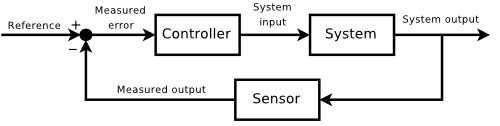
\includegraphics[width=9cm]{loop}
    \caption{Feedback loop \cite{wloop}}
    \label{fig:loop}
\end{figure}

We have chosen discrete version of PID controller because of it's simplicity and
easiness of implementation however this type of controller is meant to be used
with identified linear systems and we know that our system is not linear and we
have no means to identify it. We assumed that the robot will behave linearly
close to point of equilibrium since the equations describing the system can
linearized using Taylor series and terms with power of two and higher could be
neglected.

Standard form of PID controller look is

\begin{equation} \label{eq:pid}
    u(t) = K \left( e(t) + \frac{1}{T_i} \int_0^t e(\tau)d\tau + T_d
        \frac{de(t)}{dt} \right)
\end{equation}

\noindent where $e(t)$ is the error, the difference between required value and
the output of the system and $u(t)$ is the controller output. Performing Laplace
transformation \cite{lt} on (\ref{eq:pid}) we get

\begin{equation}
    G(s) = K \left( 1 + \frac{1}{sT_i} + sT_d \right)
\end{equation}

\noindent or the parallel form

\begin{equation} \label{eq:para}
    u(t) =  K_pe(t) + K_i \int_0^t e(\tau)d\tau + K_d
        \frac{de(t)}{dt}\end{equation}

\noindent with its Laplace transform

\begin{equation}
    G(s) = K_p + \frac{K_i}{s} + sK_d
\end{equation}

\noindent where we can simple convert the constants $K_p = K$, $K_i =
\frac{K}{T_i}$ and $K_d = KT_d$. These constants, sometimes denoted $P$, $I$, $D$ are the proportional gain,
integral time and the derivative time respectively.

\begin{figure}[h]
    \centering
    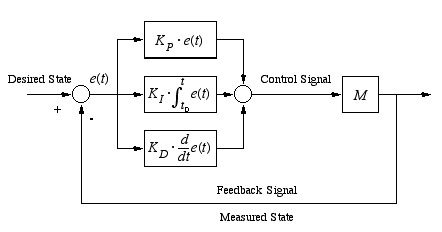
\includegraphics[width=8cm]{pid}
    \caption{PID controller in controll loop \cite{pidpic}}
    \label{fig:pidpic}
\end{figure}

Since we need to use the controller in digital form we need to use discrete form
of PID controller sometimes called PSD controller with S denoting sum instead of
integral. This can be achieved with Z-transform of the equation (\ref{eq:para}).
\cite{zt}

\begin{equation}
    U(z) = \left( K_p + \frac{K_i}{1-z^{-1}} + K_d\left(1-z^{-1}\right) \right)E(z)
\end{equation}

\begin{equation} \label{eq:zpid}
    U(z) = \left( \frac{\left( K_p + K_i + K_d\right) + \left(
    -K_p-2K_d\right)z_{-1} + K_dz^{-2}}{1-z^{-1}} \right)E(z)
\end{equation}

\noindent We have defined

\begin{eqnarray*}
    K_1 &=& K_p + K_i + K_d \\
    K_2 &=& -K_p-2K_d \\
    K_3 &=& K_d
\end{eqnarray*}

\noindent to be able to derive difference equation from (\ref{eq:zpid}).

\begin{equation}
    u[k] = u[k-1] + K_1e[k]+K_2e[k-1]+K_3e[k-2]
\end{equation}

In our final implementation of PSD controller we used slightly different
equations that incorporate also the sampling rate parameter $T_s$.

\section{Bluetooth}

\section{Scheduling}

\section{Conclusion}

\printbibliography

\end{document}
